 \subsection{Der Prototyp}
Der Prototyp der \ac{rltanzeige} ist funktionsfähig in Abb.~\ref{fig:tdot_anzeige} (siehe Kapitel \ref{rltanzeige_tdot_kapitel}) zu sehen. In diesem Abschnitt wird kurz der Aufbau dieses Prototyps (siehe Abb.~\ref{fig:rlt_anzeige_prototyp}) erklärt. 

\begin{figure}[H]
    \begin{subfigure}[l]{0.48\textwidth}
        \centering
        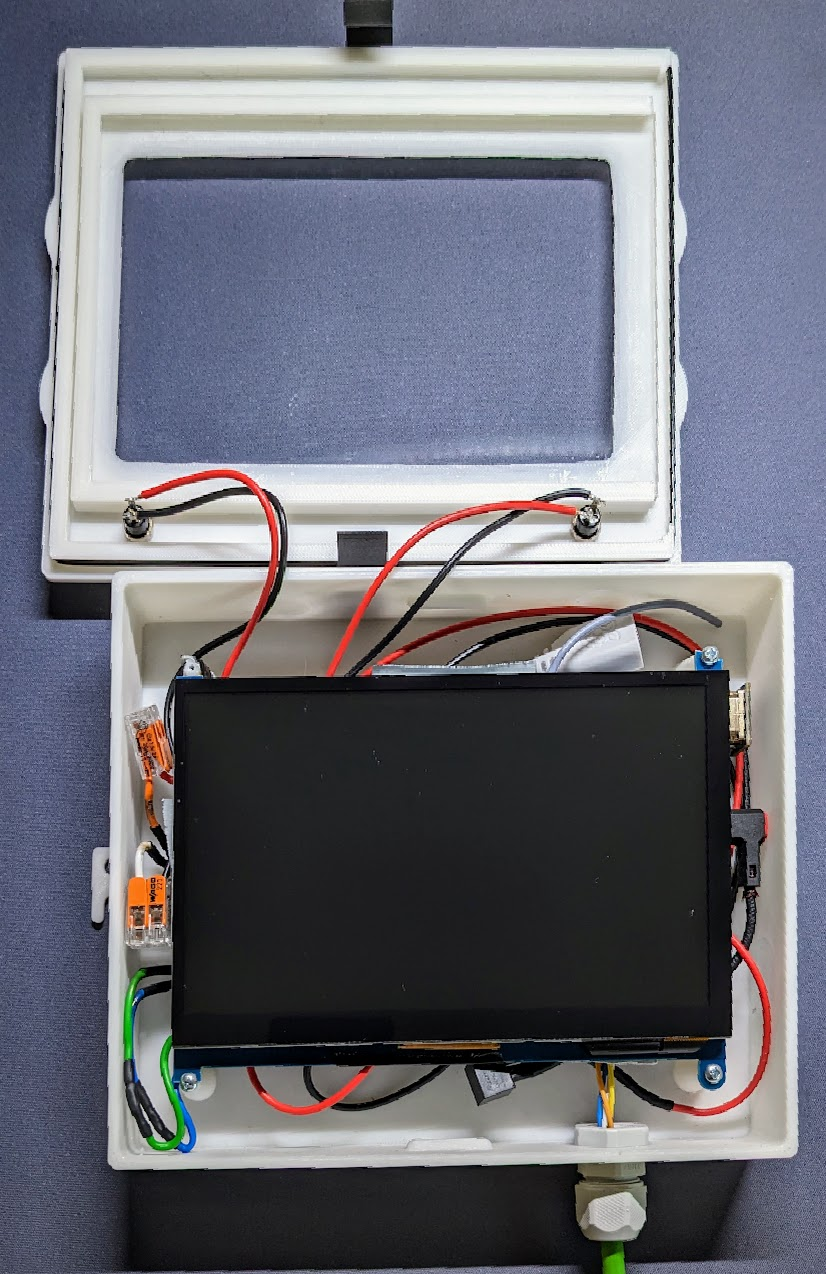
\includegraphics[width=0.99\textwidth]{prototyp_offen_w_display}
        \caption{Prototyp mit eingebautem Display \label{fig:prototyp_w_display}}
    \end{subfigure}
    \hfill
    \begin{subfigure}[r]{0.504\textwidth}
        \centering
        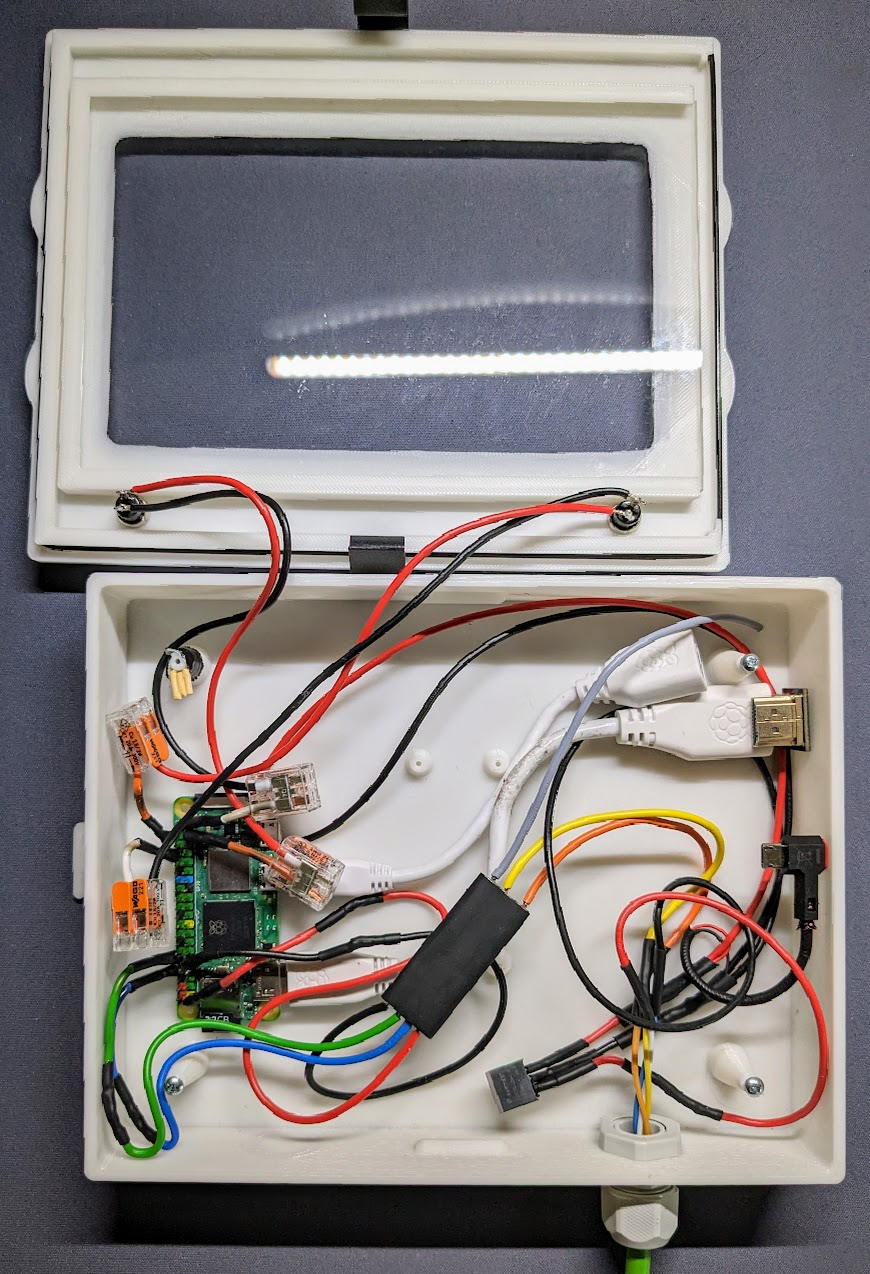
\includegraphics[width=0.99\textwidth]{prototyp_offen_w_o_display}
        \caption{Prototyp mit ausgebautem Display \label{fig:prototyp_w_o_display}}
    \end{subfigure}
	\caption{Prototyp der \ac{rltanzeige} von innen \label{fig:rlt_anzeige_prototyp}}
\end{figure}

Das Gehäuse des Prototyps ist 3D-gedruckt, um schnell Anpassungen machen zu können und nicht von einem vorgefertigten Gehäuse eingeschränkt zu werden. In diesem Gehäuse sind folgende Komponenten verbaut:

\begin{itemize}
    \item Der \textbf{Raspberry PI Zero 2 W} (siehe Abb.~\ref{fig:zero_2_w}) dient aufgrund seiner kleinen Größe und Rechenleistung als Rechner. Die Unterstützung von WLAN und Bluetooth lässt außerdem Raum zur Weiterentwicklung der \ac{rltanzeige}.
    \begin{figure}[H]
        \centering
        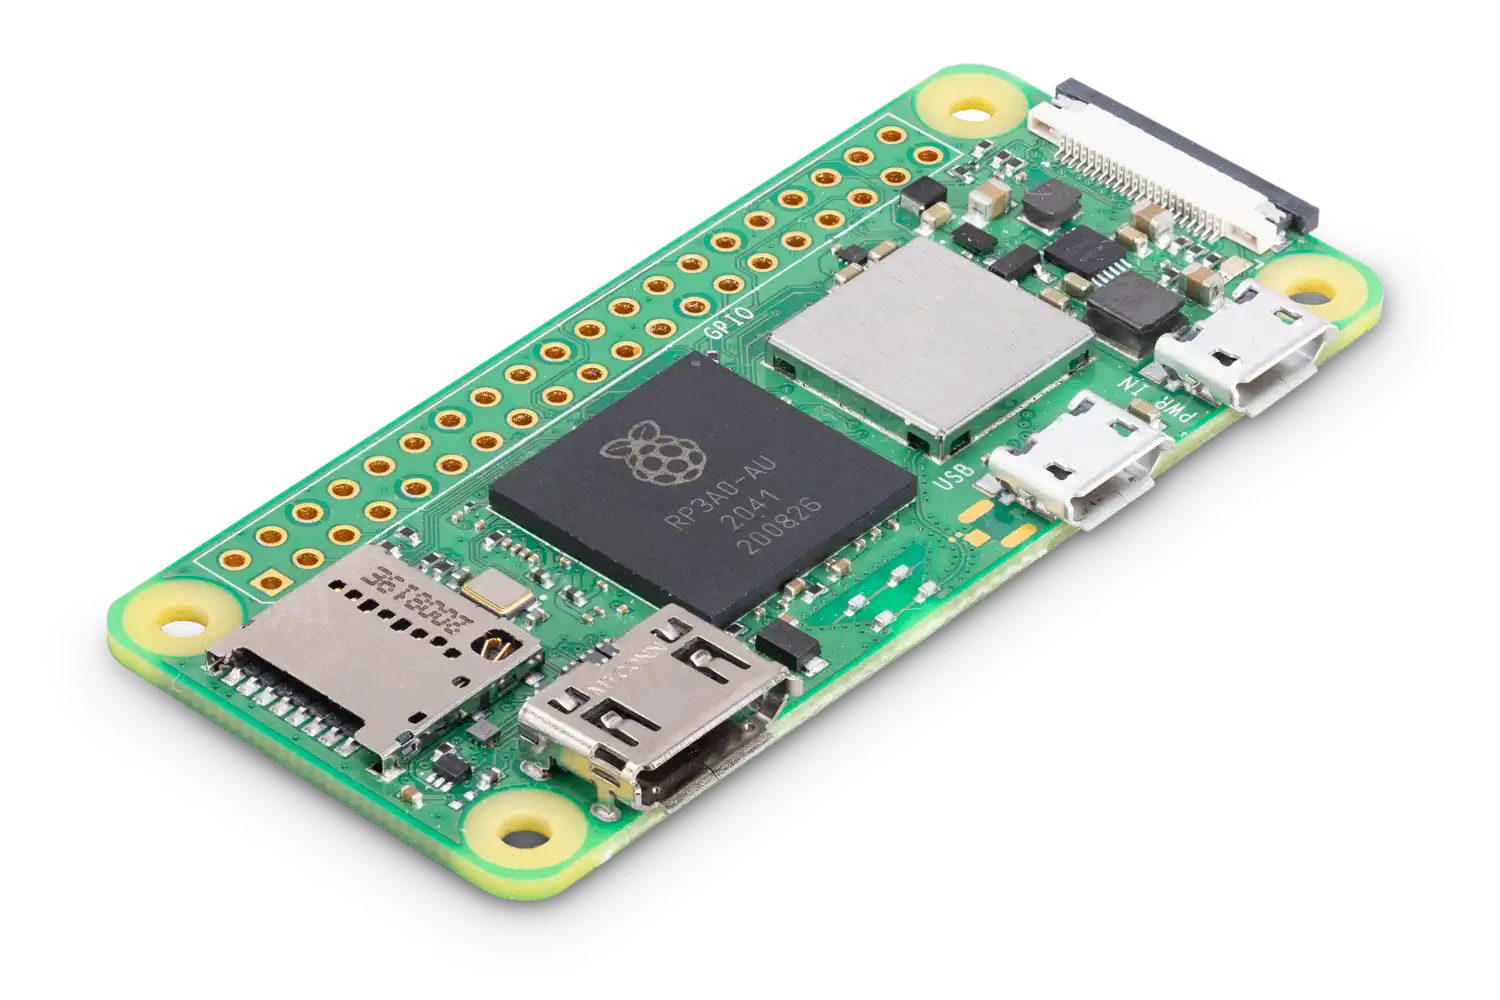
\includegraphics[width=7cm]{zero2-hero}
        \caption{Raspberry PI Zero 2 W (Quelle: \url{https://www.raspberrypi.com/products/raspberry-pi-zero-2-w/}) \label{fig:zero_2_w}}
    \end{figure}
    
    \item Das \textbf{7-Zoll Display} wird über \ac{hdmi} mit dem Raspberry PI verbunden und über Micro-USB mit Strom versorgt.

    \item Der \textbf{\ac{uart} zu \gls{gls_rs485} Adapter} (siehe Abb.~\ref{fig:ttl_rs485_adapter}) dient als Zwischenstück zwischen dem Raspberry PI und dem Bussystem. So kann das \gls{gls_rs485} Kabel mit den \ac{uart} Pins des Raspberry PIs verbunden werden.
    \begin{figure}[H]
        \centering
        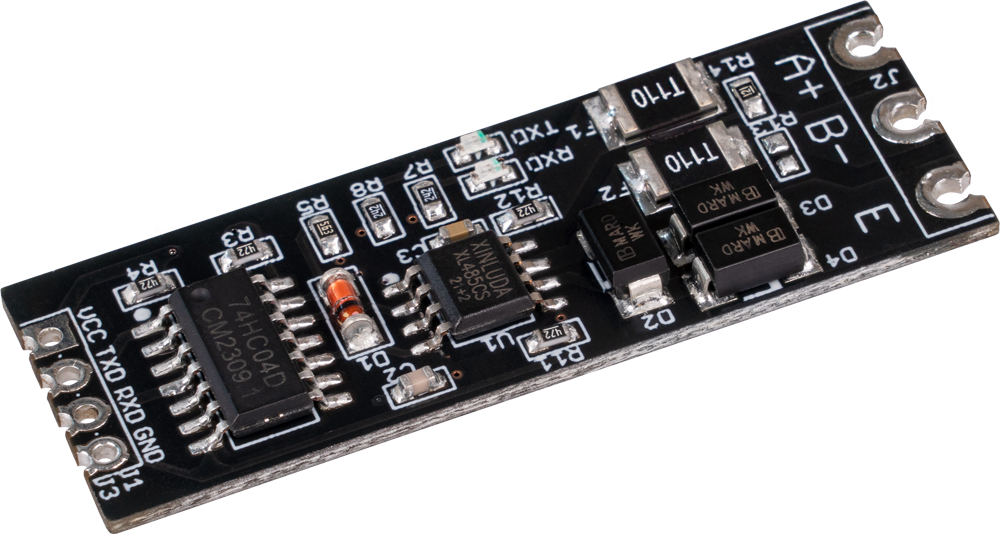
\includegraphics[width=6cm]{COM-TTL-RS4851}
        \caption{Joy-IT \ac{uart} TTL - \gls{gls_rs485} Konverter (Quelle: \url{https://joy-it.net/de/products/COM-TTL-RS485}) \label{fig:ttl_rs485_adapter}}
    \end{figure}

    \item Der \textbf{Spannungswandler} (siehe Abb.~\ref{fig:spannungswandler}) \bzw DC/DC Wandler wird benötigt, um die eingehende Spannung von 24 V auf 5 V zu reduzieren. Dabei werden sowohl der Raspberry PI als auch das Display von dieser Stromquelle versorgt.
    \begin{figure}[H]
        \centering
        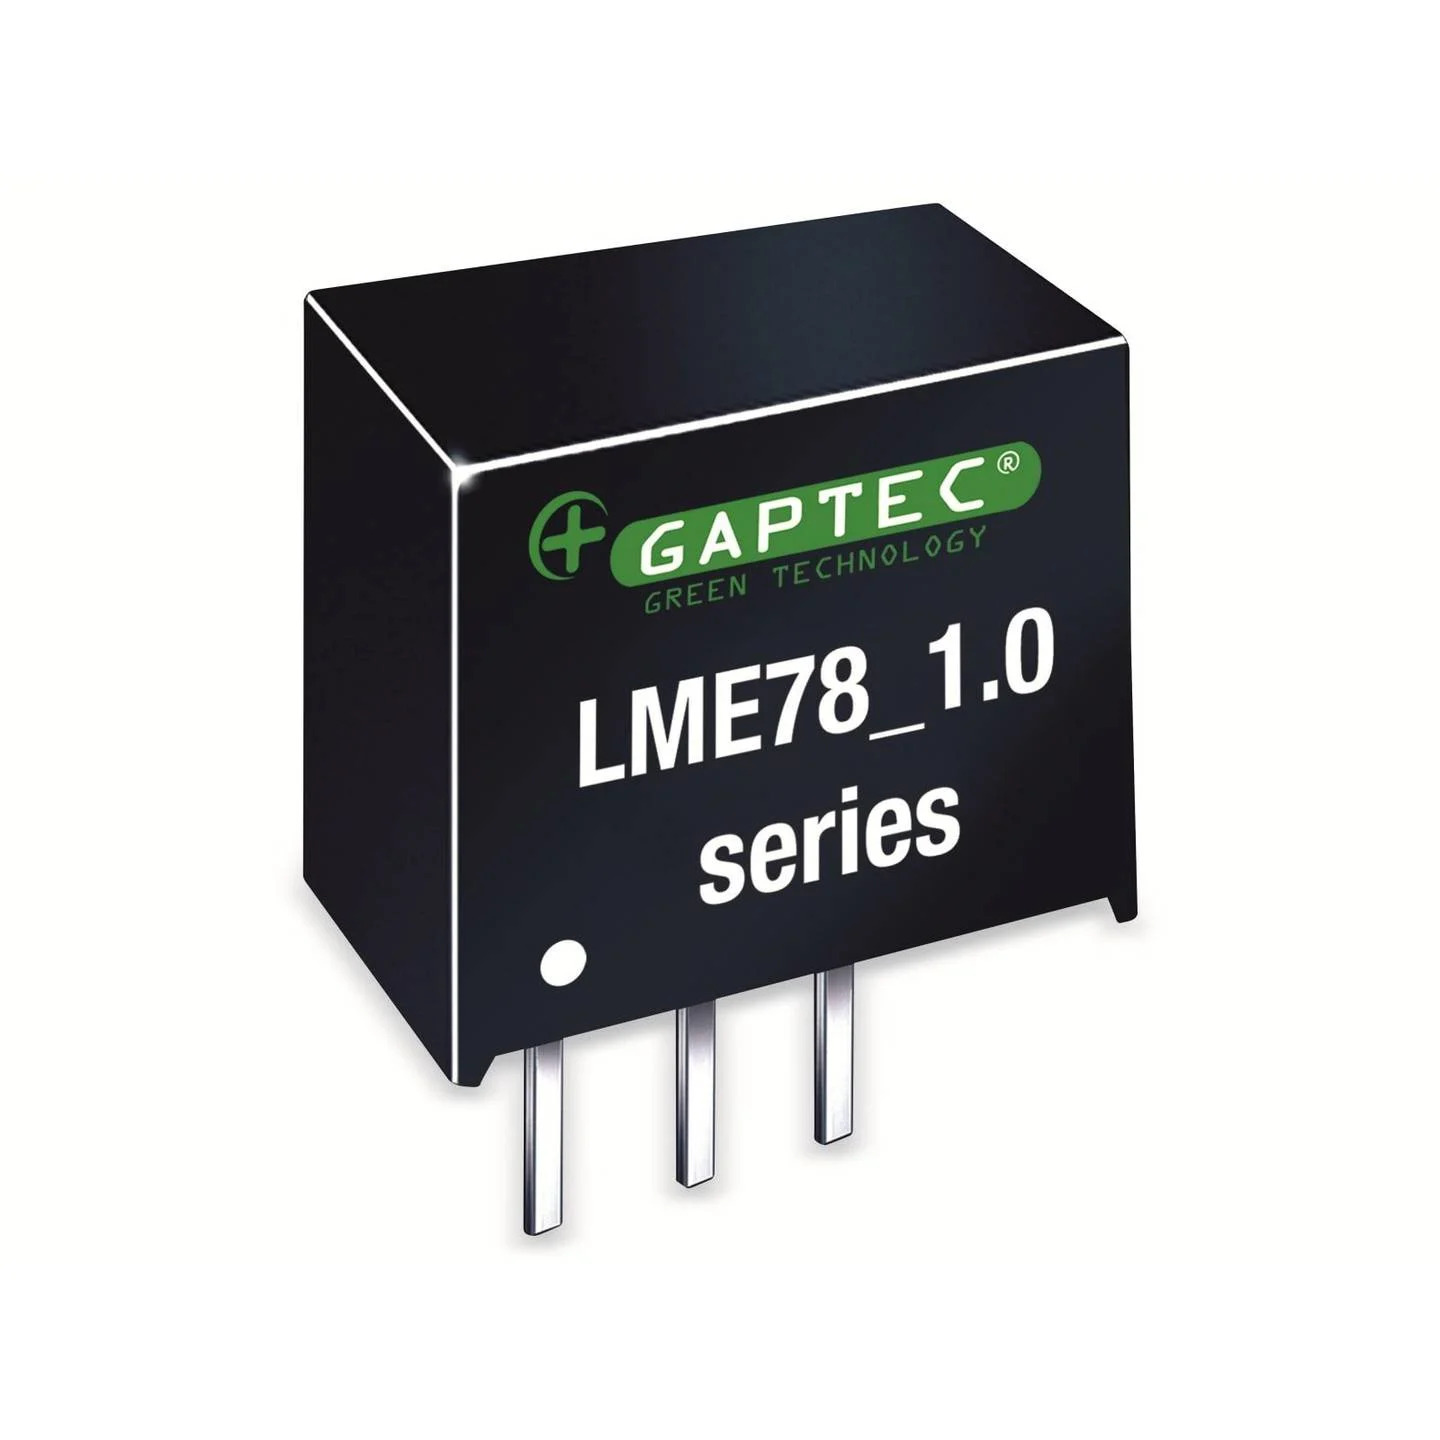
\includegraphics[width=5cm]{spannungswandler}
        \caption{Gaptec LME78\_05-1.0 DC/DC Wandler (Quelle: \url{https://www.conrad.de/de/p/gaptec-dc-dc-wandler-electronic-sip3-8-36vin-5vout-1000ma-11-6x8x10-4mm-856967933.html}) \label{fig:spannungswandler}}
    \end{figure}
\end{itemize}